\documentclass[conference,a4paper]{IEEEtran}

%% -- Packages ----------------------------------------------------
\usepackage{cite}
\usepackage{amsmath,amssymb,amsfonts}
\usepackage{algorithmic}
\usepackage{graphicx}
\usepackage{textcomp}
\usepackage{xcolor}
\usepackage{booktabs}
\usepackage{array}
\usepackage{microtype}
\usepackage{multirow}
\usepackage{float}
\usepackage{placeins}
\usepackage{url}
% Clickable citations and internal cross-references without colored boxes.
% Load hyperref last so it can patch \cite, \ref, and bibliography links.
\usepackage[hidelinks]{hyperref}

%% ── Macros & Compatibility Shims ───────────────────────────────
\def\BibTeX{{\rm B\kern-.05em{\sc i\kern-.025em b}\kern-.08em
    T\kern-.1667em\lower.7ex\hbox{E}\kern-.125emX}}
\newcommand{\cmark}{\ensuremath{\checkmark}}
\newcommand{\xmark}{\ensuremath{-}}
\providecommand{\Description}[1]{}

\begin{document}

%% ════════════════════════════════════════════════════════════════
%%  TITLE AND AUTHORS
%% ════════════════════════════════════════════════════════════════
\title{Multi-Stage Compression of Small Language Models for Energy-Efficient Inference: An Empirical Systems Ablation}

\author{
\IEEEauthorblockN{Md. Sadik Shahriar}
\IEEEauthorblockA{\textit{Department of Computer Science and Engineering} \\
\textit{East West University}\\
Dhaka, Bangladesh \\
shahriarsadik@gmail.com}
\and
\IEEEauthorblockN{Nipa Mridha}
\IEEEauthorblockA{\textit{Department of Computer Science and Engineering} \\
\textit{East West University}\\
Dhaka, Bangladesh \\
mridhanipa886@gmail.com}
\and
\IEEEauthorblockN{Tanha Humaira}
\IEEEauthorblockA{\textit{Department of Computer Science and Engineering} \\
\textit{East West University}\\
Dhaka, Bangladesh \\
chandnihumaira373@gmail.com}
\and
\IEEEauthorblockN{Ahmed Abdal Shafi Rasel}
\IEEEauthorblockA{\textit{Department of Computer Science and Engineering} \\
\textit{East West University}\\
Dhaka, Bangladesh \\
ahmed.shafi@ewubd.edu}
}


\maketitle

%% ════════════════════════════════════════════════════════════════
%%  ABSTRACT
%% ════════════════════════════════════════════════════════════════
\begin{abstract}
Deploying small language models (SLMs) on power-constrained hardware requires balancing energy consumption, memory footprint, decode throughput, and accuracy. We measure the physical interactions, operating boundaries, and realization gaps of stacked weight quantization, token eviction, and KV-cache quantization on a 70~W NVIDIA T4 server GPU across context lengths of 1024, 2048, and 4096 tokens, with board power logged at 10~Hz via NVML. Quality is evaluated using a calibrated 60-scenario hard-retrieval benchmark requiring exact-match UUID extraction at 4096 tokens across three insertion depths.

The measured trade-offs vary with model and sequence length. On Llama~3.2-3B (3:1 GQA), combining 4-bit AWQ with custom PyramidKV eviction provides the best overall trade-off at 4096 tokens: relative to stock AWQ, total energy decreases by 101.95~J (16.15\%), active KV cache drops by 73.8\% (455 to 119~MiB), and decode throughput increases by 47.7\% (13.77 to 20.34~tok/s). Retrieval remains within one scenario of wrapped AWQ (37/60 vs.\ 38/60). The same policy on Qwen2.5-3B (8:1 GQA) reduces accuracy from 48/60 to 1/60, with limited recovery after a 50\% budget increase. A negative interaction ($I < 0$) indicates that prior eviction reduces the incremental energy cost of reference quantization. Finally, the evaluated TurboQuant implementation retains uncompressed tensors alongside discrete indices, increasing active cache storage by over 50\%. The findings characterize T4 inference, with separate measurements needed for edge devices.
\end{abstract}

%% ── Keywords ───────────────────────────────────────────────────
\begin{IEEEkeywords}
Energy-efficient inference, Green AI, KV-cache compression, model compression, small language models
\end{IEEEkeywords}

%% ════════════════════════════════════════════════════════════════
%%  1. INTRODUCTION
%% ════════════════════════════════════════════════════════════════
\section{Introduction}

Deploying small language models (SLMs) on resource-constrained hardware requires balancing energy consumption, memory footprint, decode throughput, and accuracy~\cite{strubell_energy_2019,patterson_carbon_2021,schwartz2020green}. The key-value (KV) cache grows linearly with context length, increasing memory demands during autoregressive generation~\cite{li2024survey,dao_flashattention_2022}. Models under 4B parameters offer an attractive physical profile for local hosting~\cite{husom_sustainable_2025}. Measuring stacked compression on small models is important because quantization sensitivity varies across architectures~\cite{wang_slmquant_2025}.

Prior work targets memory traffic through three mechanisms: 4-bit weight quantization such as AWQ~\cite{lin_awq_2025}, token eviction heuristics such as PyramidKV, SnapKV, and H2O~\cite{cai_pyramidkv_2025,li_snapkv_2024,zhang_h2o_2023}, and KV-cache quantization methods such as TurboQuant, KIVI, and JanusQuant~\cite{zandieh2026turboquant,liu_kivi_2023,sun2026janusquant}. RDKV~\cite{zhang_rdkv_2026} and ThinKV~\cite{ramachandran_thinkv_2026} combine eviction and KV quantization. Yet empirical silicon data for stacked pipelines on compact architectures remains scarce. We address this gap through an empirical systems study on a server-class NVIDIA T4 GPU, evaluating sequential combinations of AWQ, custom PyramidKV eviction, and TurboQuant on Llama~3.2-3B-Instruct and Qwen2.5-3B-Instruct, continuously polling board power at 10~Hz via NVML~\cite{argerich_watt_2026,nvidia2024nvml}.

\paragraph{Research Questions}
We investigate four core questions:
\begin{itemize}
\item \textbf{RQ1 (Context Scaling and Efficiency):} How do weight quantization, token eviction, and KV-cache quantization affect physical GPU energy consumption and decode throughput across 1024, 2048, and 4096 tokens?
\item \textbf{RQ2 (Cross-Architectural Robustness):} How does the same token eviction policy affect retrieval on Llama and Qwen, and how sensitive is Qwen to the retained-token budget?
\item \textbf{RQ3 (Compound Interaction and Shielding):} When multiple compression stages are applied sequentially, do their energy effects add up or is there an energetic shielding interaction?
\item \textbf{RQ4 (Multi-Objective Pareto Optimization):} Which compression configurations define the non-dominated Pareto frontier across energy, accuracy, throughput, and memory under bootstrap resampling?
\end{itemize}

\paragraph{Key Contributions}
The main empirical discoveries of this work are:
\begin{enumerate}
\item \textbf{Limits of Sequential Stacking:} The tested compression stages have non-additive energy effects on the T4. On Llama~3.2-3B, single-stage token eviction + AWQ achieved the best trade-off at 4096 tokens: a 101.95~J (16.15\%) total energy reduction relative to stock AWQ, a 47.7\% throughput improvement (13.77 to 20.34~tok/s), a 73.8\% smaller active cache (455 to 119~MiB), and retrieval accuracy within one scenario of wrapped AWQ (37/60 vs.\ 38/60). Adding sequential quantization slowed execution and increased energy.
\item \textbf{Model Sensitivity to Eviction:} The eviction policy that preserved retrieval on Llama (3:1 GQA) reduced accuracy to 1/60 on Qwen2.5-3B (8:1 GQA). Expanding the retained-token budget by 50\% raised Qwen retrieval from 1/15 to 2/15 on the same scenarios. The difference across models motivates a controlled study of GQA head sharing~\cite{ainslie2023gqa}.
\item \textbf{Upstream Overhead Shielding:} Both models showed negative energy interaction contrasts ($I < 0, p < 0.01$). Qwen used a matched wrapper, and Llama retained the negative sign in a separate baseline sensitivity check. The result is consistent with quantization operating on a smaller cache after eviction.
\item \textbf{Realization Gaps in Reference Implementations:} Off-the-shelf reference code can diverge sharply from algorithmic theory. TurboQuant's reference implementation added 31\% to 45\% energy overhead while allocating uncompressed FP16 tensors alongside index tables, expanding memory footprint rather than reducing it.
\end{enumerate}

%% ════════════════════════════════════════════════════════════════
%%  2. RELATED WORK
%% ════════════════════════════════════════════════════════════════
\section{Related Work}

\paragraph{Weight and Cache Quantization}
Weight quantization reduces static model storage and transfer bandwidth. AWQ~\cite{lin_awq_2025} protects activation-salient channels during 4-bit rounding, while GPTQ~\cite{frantar_gptq_2023} relies on second-order error compensation. Both target model weights, so their results leave open the cost of adding KV-cache compression. SLMQuant~\cite{wang_slmquant_2025} showed that compact sub-4B models exhibit greater quantization sensitivity than larger LLMs, demonstrating that target architectures require direct hardware evaluation. For the KV cache, TurboQuant~\cite{zandieh2026turboquant} applies random orthogonal rotations followed by scalar quantization without calibration data. KIVI~\cite{liu_kivi_2023} employs 2-bit per-channel key and per-token value quantization, and JanusQuant~\cite{sun2026janusquant} targets long-sequence contexts. Salfati~\cite{salfati_quantization_2026} shows how to optimize value projection under fixed attention and identifies equal-storage comparisons with cache quantization as open. These studies motivate measuring the realized storage and energy of a low-bit reference implementation.

\paragraph{Token Eviction and Energy Measurement}
Token eviction prunes cache entries to bound memory use. H2O~\cite{zhang_h2o_2023} demonstrated that retaining attention heavy hitters can preserve generation quality. SnapKV~\cite{li_snapkv_2024} selects prompt tokens using an observation window, and PyramidKV~\cite{cai_pyramidkv_2025} validates layer-dependent budgets on LongBench and needle retrieval. Those tests leave the portability of a custom PyramidKV-style policy across AWQ 3B models open. RDKV~\cite{zhang_rdkv_2026} jointly allocates precision and eviction, includes a sequential baseline, and reports latency and memory with packed decoding. ThinKV~\cite{ramachandran_thinkv_2026} adapts eviction and quantization to reasoning workloads. Watt Counts~\cite{argerich_watt_2026} compares inference energy across GPUs, and Husom et al.~\cite{husom_sustainable_2025} analyze edge inference scaling. Our study measures how stacking fixed AWQ, eviction, and reference quantization stages changes board energy for two 3B models on the same T4 platform.

%% ════════════════════════════════════════════════════════════════
%%  3. METHODOLOGY AND BENCHMARK DESIGN
%% ════════════════════════════════════════════════════════════════
\section{Methodology and Benchmark Design}

Figure~\ref{fig:methodology} illustrates our experimental workflow across model configurations, power profiling, benchmark evaluation, and statistical validation.

\begin{figure}[t]
\centering
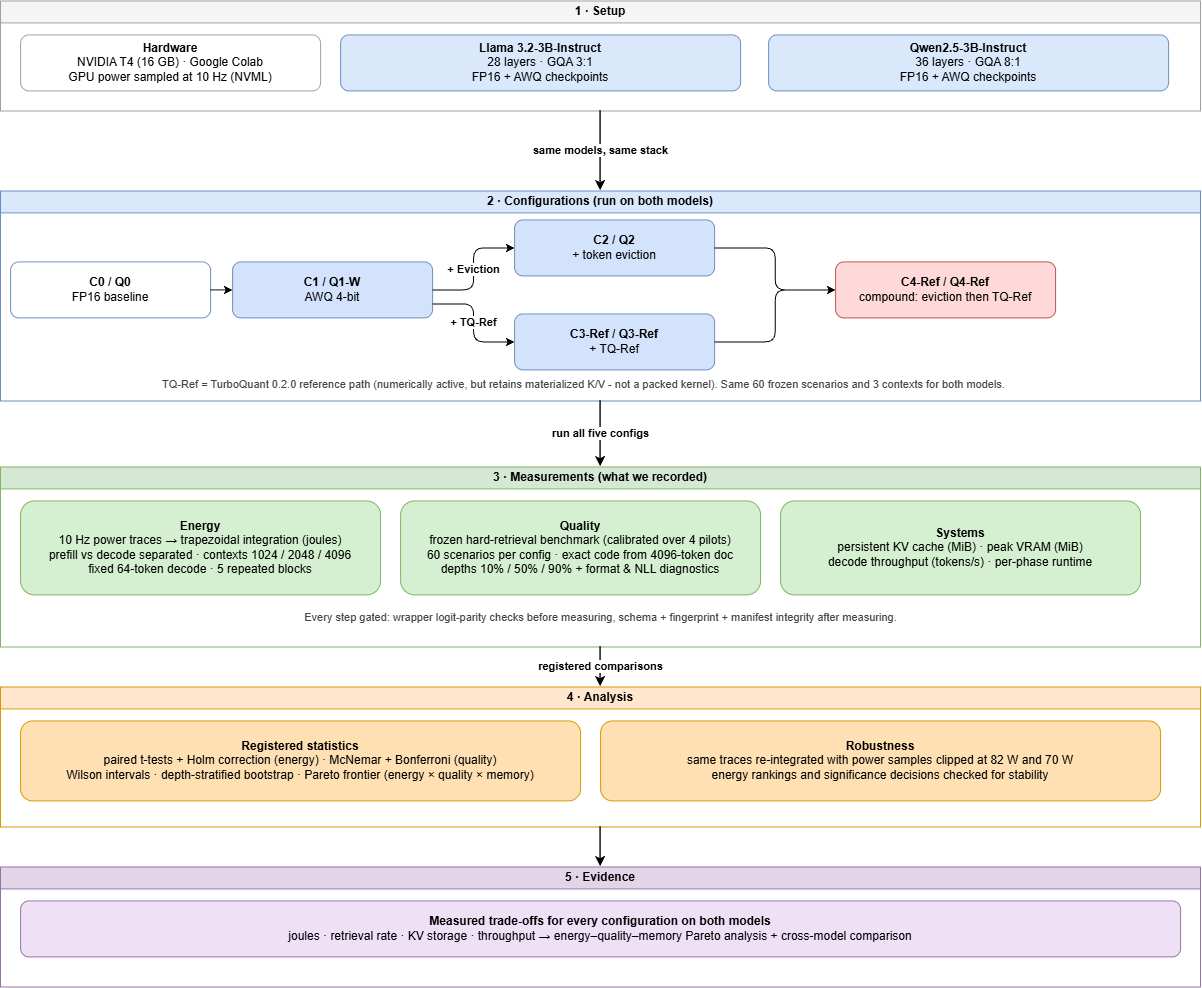
\includegraphics[width=0.60\columnwidth]{figures/methodology_diagram.png}
\Description{Flowchart of the experimental workflow: five compression configurations evaluated on Llama 3.2-3B and Qwen2.5-3B, logging 10 Hz power traces, hard-retrieval quality, and system trade-offs.}
\caption{Experimental workflow for both models, including compression, 10~Hz power logging, retrieval evaluation, and system trade-off analysis.}
\label{fig:methodology}
\end{figure}

\subsection{Model Architectures and Configurations}
We evaluated two open-weight models with 3B parameters: Llama~3.2-3B-Instruct (28 layers, 24 query heads, 8 KV heads, 3:1 GQA ratio~\cite{ainslie2023gqa}, 128K configured context) and Qwen2.5-3B-Instruct (36 layers, 16 query heads, 2 KV heads, 8:1 GQA ratio, 32K configured context), both with head dimension 128. For Llama, we used the Unsloth FP16 baseline~\cite{unsloth_2024} and CasperHansen AWQ release~\cite{casperhansen_llama32_awq}. For Qwen, we used official checkpoints~\cite{qwen2024technical}. Our software environment ran PyTorch~2.11.0~\cite{paszke2019pytorch}, Transformers~5.12.1~\cite{wolf2020transformers}, and TurboQuant~0.2.0~\cite{back2matching_turboquant_v020}.

We evaluated five configurations: \textbf{(1) FP16 Baseline (C0 / Q0):} Uncompressed reference execution; \textbf{(2) AWQ Baseline (C1, C1-W / Q1-W):} 4-bit weight-only quantization without KV compression; \textbf{(3) AWQ+Eviction (C2 / Q2):} AWQ with layerwise token eviction averaging 1024 retained tokens per layer; \textbf{(4) AWQ+TQ-Ref (C3-Ref / Q3-Ref):} AWQ with numerical KV quantization; and \textbf{(5) Compound Stack (C4-Ref / Q4-Ref):} Sequential composition (AWQ $\to$ eviction $\to$ TurboQuant). Llama uses stock AWQ (C1) for the core systems runs and wrapped AWQ (C1-W) for retrieval and the separate 4096-token control. Qwen uses wrapped AWQ (Q1-W) throughout its AWQ comparisons.

\subsection{Hardware and Power Measurement Protocol}
Experiments ran on a server-class NVIDIA Tesla T4 GPU (16~GB nominal VRAM, 70~W nominal cap) on Google Colab. We polled GPU board power at 10~Hz via NVML~\cite{nvidia2024nvml} using \texttt{pynvml}, following Argerich et al.~\cite{argerich_watt_2026}. Total energy was computed by trapezoidal numerical integration over recorded power traces. All energy runs used teacher-forced decoding for exactly 64 tokens across context lengths of 1024, 2048, and 4096 tokens with five independent measurement blocks per condition ($n=5$).

\subsection{Eviction and TurboQuant Realization Audit}
Token eviction was implemented using a custom PyTorch attention wrapper. During prefill, token importance scores are computed by averaging attention weights over a 32-token observation window. We apply a layer-dependent pyramidal budget averaging 1024 retained tokens per layer (larger budgets in earlier layers, decay $\beta=20$), pruning tokens below the threshold before decoding. With compression disabled, the wrapper matched stock AWQ logits and outputs on one probe per depth for each model. This check covers baseline parity, and reproducing published PyramidKV benchmark results remains future work.

TurboQuant~\cite{zandieh2026turboquant} applies random orthogonal rotations to KV vectors and maps coordinates to discrete codebook indices. We evaluated the independent \texttt{turboquant} implementation (v0.2.0)~\cite{back2matching_turboquant_v020}. In this package, coordinates are stored as \texttt{uint8} indices while uncompressed FP16 key and value tensors remain concurrently allocated in GPU memory. Consequently, the reference path is numerically active during attention computation but does not reduce physical device memory, exposing a software-to-hardware realization gap. A packed and fused kernel achieves net energy reduction only when compute overhead remains below the memory traffic boundary: $O_\text{net} < \epsilon_\text{mem} \cdot \Delta_D$, where $\epsilon_\text{mem}$ is energy saved per byte and $\Delta_D$ is avoided decode traffic.

\subsection{Calibrated Hard-Retrieval Benchmark}
\label{sec:benchmark}
Standard downstream benchmarks probe static weights rather than KV-cache degradation, while naive synthetic needle-in-a-haystack (NIAH) tests~\cite{kamradt2023needle} saturated at 100\% across all configurations in preliminary trials. Following established KV evaluation methodology~\cite{cai_pyramidkv_2025,li_snapkv_2024,zhang_h2o_2023}, we implemented a calibrated 4096-token hard-retrieval benchmark requiring exact-match UUID key-value extraction across 60 frozen scenarios: 20 inserted at 10\% depth, 20 at 50\%, and 20 at 90\% document depth. Distractor density and key distinctiveness were calibrated across four pilot iterations so that uncompressed baselines achieved high but imperfect accuracy ($\approx 75\%-88\%$), providing headroom to detect compression loss without floor or ceiling artifacts.

\subsection{Statistical Methodology}
Energy differences were evaluated using paired two-sided $t$-tests across five measurement blocks ($n=5$), reporting 95\% confidence intervals and controlling family-wise error rates with Holm sequential step-down correction~\cite{holm1979simple}. Non-parametric Wilcoxon signed-rank tests~\cite{wilcoxon1945individual} served as secondary verification. Retrieval accuracy across the 60 benchmark scenarios was evaluated with Wilson score 95\% confidence intervals~\cite{wilson1927probable}, and paired binary accuracy differences were tested via exact McNemar tests~\cite{mcnemar1947note} with Bonferroni correction. Cross-model retrieval contrasts and Pareto frontier stability used 2000 draws stratified by retrieval depth. The frontier analysis (seed 407) resampled systems blocks jointly within sessions, drew C1-W independently, and fixed cache sizes at their observed means.

%% ════════════════════════════════════════════════════════════════
%%  4. EMPIRICAL RESULTS
%% ════════════════════════════════════════════════════════════════
\section{Empirical Results}

\subsection{Energy and Decode Throughput Across Contexts}
\label{sec:energy-scaling}

Table~\ref{tab:energy-scaling} reports total energy, decode throughput, peak allocated VRAM, and active KV-cache volume across context lengths for both models.

\begin{table}[t]
\caption{Energy, Throughput, VRAM, and Active Cache Across Contexts}
\label{tab:energy-scaling}
\centering\footnotesize
\setlength{\tabcolsep}{1.4pt}
\renewcommand{\arraystretch}{0.78}
\begin{tabular*}{\columnwidth}{@{\extracolsep{\fill}}llrrrr@{}}
\toprule
\multicolumn{6}{c}{\textbf{Llama 3.2-3B (3:1 GQA)}} \\
\midrule
\textbf{Ctx.} & \textbf{Configuration} & \textbf{$E$ (J)} & \textbf{tok/s} & \textbf{VRAM} & \textbf{Cache} \\
\midrule
1024 & FP16 (C0)          & $244.11 \pm 13.10$ & 21.09 & 8810  & 119.0 \\
     & AWQ (C1)           & $268.77 \pm 26.20$ & 18.24 & 4943  & 119.0 \\
     & Evict (C2)         & $253.61 \pm 14.36$ & 19.31 & 4920  &  92.3 \\
     & TQ-Ref (C3-Ref)    & $367.00 \pm 28.44$ & 13.49 & 5099  & 187.2 \\
     & Compound (C4-Ref)  & $364.91 \pm 21.59$ & 12.75 & 5042  & 146.8 \\
\midrule
2048 & FP16 (C0)          & $345.26 \pm 4.97$  & 17.42 & 9663  & 231.0 \\
     & AWQ (C1)           & $313.81 \pm 9.31$  & 20.13 & 5795  & 231.0 \\
     & Evict (C2)         & $338.74 \pm 21.03$ & 17.81 & 5691  & 119.0 \\
     & TQ-Ref (C3-Ref)    & $439.58 \pm 9.11$  & 13.33 & 6116  & 357.0 \\
     & Compound (C4-Ref)  & $435.05 \pm 24.47$ & 12.87 & 5853  & 187.2 \\
\midrule
4096 & FP16 (C0)          & $701.08 \pm 8.12$  & 11.34 & 12688 & 455.0 \\
     & AWQ (C1)           & $631.25 \pm 5.05$  & 13.77 & 8820  & 455.0 \\
     & Evict (C2)         & $529.30 \pm 20.02$ & 20.34 & 8500  & 119.0 \\
     & TQ-Ref (C3-Ref)    & $913.48 \pm 2.11$  &  7.66 & 9468  & 696.5 \\
     & Compound (C4-Ref)  & $659.50 \pm 21.35$ & 12.53 & 8662  & 187.2 \\
\midrule
\multicolumn{6}{c}{\textbf{Qwen2.5-3B (8:1 GQA)}} \\
\midrule
\textbf{Ctx.} & \textbf{Configuration} & \textbf{$E$ (J)} & \textbf{tok/s} & \textbf{VRAM} & \textbf{Cache} \\
\midrule
1024 & FP16 (Q0)          & $258.57 \pm 27.40$ & 19.73 & 8061 &  38.2 \\
     & AWQ (Q1-W)         & $293.42 \pm 21.61$ & 12.11 & 4273 &  38.2 \\
     & Evict (Q2)         & $272.02 \pm 13.92$ & 12.91 & 4264 &  29.7 \\
     & TQ-Ref (Q3-Ref)    & $358.58 \pm 9.61$  &  9.60 & 4321 &  60.2 \\
     & Compound (Q4-Ref)  & $342.96 \pm 14.14$ &  9.76 & 4299 &  47.3 \\
\midrule
2048 & FP16 (Q0)          & $334.15 \pm 17.52$ & 17.87 & 8149 &  74.2 \\
     & AWQ (Q1-W)         & $398.46 \pm 12.46$ & 13.70 & 4350 &  74.2 \\
     & Evict (Q2)         & $342.56 \pm 10.34$ & 12.78 & 4297 &  38.2 \\
     & TQ-Ref (Q3-Ref)    & $540.87 \pm 14.11$ &  8.94 & 4436 & 114.8 \\
     & Compound (Q4-Ref)  & $435.18 \pm 20.00$ &  9.10 & 4343 &  60.2 \\
\midrule
4096 & FP16 (Q0)          & $616.78 \pm 6.79$  & 13.23 & 8249 & 146.2 \\
     & AWQ (Q1-W)         & $621.75 \pm 25.14$ & 13.12 & 4460 & 146.2 \\
     & Evict (Q2)         & $550.48 \pm 10.07$ & 12.53 & 4297 &  38.2 \\
     & TQ-Ref (Q3-Ref)    & $812.28 \pm 13.11$ &  8.54 & 4668 & 223.9 \\
     & Compound (Q4-Ref)  & $628.69 \pm 9.77$  &  9.04 & 4343 &  60.2 \\
\bottomrule
\end{tabular*}

\vspace{1pt}
\raggedright\footnotesize $E$ is mean $\pm$ SD; VRAM and cache are in MiB.\par
\end{table}

\paragraph{Context-Dependent Scaling}
On Llama, stock AWQ (C1) consumed 24.66~J more energy than FP16 at 1024 tokens due to dequantization overhead on short sequences. At 4096 tokens, AWQ achieved a 9.96\% energy reduction (631.25~J vs.\ 701.08~J) as parameter bandwidth savings offset kernel overhead. On Qwen, AWQ produced no net savings over FP16 across any context length (621.75~J vs.\ 616.78~J at 4096 tokens).

\paragraph{Long-Context Eviction and Statistical Significance}
At 4096 tokens on Llama, token eviction (C2) produced substantial multi-dimensional improvements over stock AWQ (C1): reducing total energy by 101.95~J (16.15\%, $529.30$ vs.\ $631.25$~J, paired $t$-test Holm $p = 0.00549$, 95\% CI: $[73.81, 130.08]$~J), accelerating decode throughput from 13.77 to 20.34~tok/s (47.7\% speedup), and reducing active cache volume by 73.8\% (455 to 119~MiB). Conversely, TurboQuant reference (C3-Ref) increased Llama energy by 282.24~J relative to stock AWQ (95\% CI: $[277.25, 287.23]$~J, $p = 1.9 \times 10^{-7}$). TQ-Ref used 913.48~J on Llama and 812.28~J on Qwen, with throughput of 7.66 and 8.54~tok/s, respectively. Compound stacking (C4-Ref, 659.50~J) did not differ significantly from the AWQ baseline ($-28.26$~J, $p = 0.2465$), but consumed significantly more energy than eviction alone ($-130.21$~J, $p = 0.00620$) and significantly less than standalone TurboQuant ($+253.98$~J, $p = 0.000206$).

\subsection{Sequential Interaction and Overhead Shielding}
\label{sec:interaction}
To evaluate how multi-stage compression interacts when stacked sequentially, we define the Llama interaction contrast $I = (\text{C4-Ref} - \text{C3-Ref}) - (\text{C2} - \text{C1})$ using configuration energies. A negative interaction ($I < 0$) indicates lower incremental quantization energy after eviction. With stock AWQ, $I = -152.03$~J (95\% CI: $[-187.11, -116.96]$~J, Holm $p = 0.00109$). At 4096 tokens, stock C1 averaged $631.25 \pm 5.05$~J and wrapped C1-W averaged $639.86 \pm 5.48$~J (mean $\pm$ SD), a difference of $+8.61$~J (1.36\%). Substituting the wrapped mean shifts $I$ to $-143.42$~J. The control used a separate session and a different prompt, so the substitution is descriptive. Qwen's within-session, wrapper-matched interaction was $-112.32$~J (95\% CI: $[-147.36, -77.28]$~J, Holm $p = 0.00352$).

\subsection{Hard-Retrieval Quality and Depth Analysis}

Table~\ref{tab:quality} reports exact-match retrieval accuracy across the 60 benchmark scenarios broken down by insertion depth.

\begin{table}[t]
\caption{Hard-Retrieval Accuracy and Depth Breakdown at 4096 Tokens (60 Scenarios per Configuration)}
\label{tab:quality}
\centering\footnotesize
\setlength{\tabcolsep}{0.4pt}
\renewcommand{\arraystretch}{0.80}
\begin{tabular*}{\columnwidth}{@{\extracolsep{\fill}}llccccr@{}}
\toprule
\textbf{Model} & \textbf{Config.} & \textbf{10\%} & \textbf{50\%} & \textbf{90\%} & \textbf{Total} & \textbf{95\% CI} \\
\midrule
\shortstack[l]{Llama\\(3:1 GQA)} & FP16 (C0)      & 19/20 & 13/20 & 15/20 & 47/60 (78.3\%) & $[.664,.869]$ \\
               & AWQ (C1-W)             & 18/20 & 10/20 & 10/20 & 38/60 (63.3\%) & $[.507,.744]$ \\
               & Eviction (C2)          & 18/20 & 10/20 &  9/20 & 37/60 (61.7\%) & $[.490,.729]$ \\
               & TQ-Ref (C3-Ref)        & 18/20 & 10/20 &  9/20 & 37/60 (61.7\%) & $[.490,.729]$ \\
               & Compound (C4-Ref)      & 17/20 & 10/20 & 10/20 & 37/60 (61.7\%) & $[.490,.729]$ \\
\midrule
\shortstack[l]{Qwen\\(8:1 GQA)} & FP16 (Q0)      & 20/20 & 17/20 & 16/20 & 53/60 (88.3\%) & $[.778,.942]$ \\
               & AWQ (Q1-W)             & 18/20 & 15/20 & 15/20 & 48/60 (80.0\%) & $[.682,.882]$ \\
               & Eviction (Q2)          &  0/20 &  0/20 &  1/20 &  1/60 (1.7\%)  & $[.003,.089]$ \\
               & TQ-Ref (Q3-Ref)        & 18/20 & 16/20 & 15/20 & 49/60 (81.7\%) & $[.701,.894]$ \\
               & Compound (Q4-Ref)      &  0/20 &  0/20 &  1/20 &  1/60 (1.7\%)  & $[.003,.089]$ \\
\bottomrule
\end{tabular*}
\end{table}

\paragraph{Llama Stability vs.\ Qwen Eviction Collapse}
On Llama, eviction (C2), TurboQuant (C3-Ref), and compound stacking (C4-Ref) each achieved 37/60 (61.7\%), differing from the AWQ baseline (38/60) by only one test case (exact McNemar $p = 1.0$). On Qwen, single-stage eviction (Q2) caused retrieval accuracy to collapse from 48/60 down to 1/60 (Bonferroni-adjusted McNemar $p = 1.71 \times 10^{-13}$). Compound stacking (Q4-Ref) inherited this failure (1/60). In contrast, TurboQuant reference (Q3-Ref) preserved retrieval fidelity (49/60 vs.\ 48/60 on Q1-W). The cross-model eviction contrast $(\Delta_{\text{Qwen}} - \Delta_{\text{Llama}})$ was $-0.767$ (bootstrap 95\% CI: $[-0.867, -0.667]$).

\subsection{Qwen Sensitivity Sweeps}
Table~\ref{tab:qwen-sensitivity} presents sensitivity sweeps on Qwen at 4096 tokens across 15 common scenarios. Increasing the retained-token budget by 50\% (from 1024 to 1536 tokens) raised retrieval from 1/15 to 2/15 on the same scenarios, showing limited recovery over the tested budgets. In bit-width sweeps, 2-bit quantization caused notable accuracy degradation (4/15), whereas 3-bit (11/15) and 4-bit (12/15) maintained strong retrieval fidelity.

\begin{table}[t]
\caption{Qwen Sensitivity Sweeps at 4096 Tokens (15 Common Test Scenarios)}
\label{tab:qwen-sensitivity}
\centering\footnotesize
\setlength{\tabcolsep}{3pt}
\renewcommand{\arraystretch}{0.80}
\begin{tabular}{@{}l rrc@{}}
\toprule
\textbf{Variant} & \textbf{Total Energy (J)} & \textbf{Retrieval} & \textbf{Wilson 95\% CI} \\
\midrule
\multicolumn{4}{@{}l}{\textit{PyramidKV Token Budget Sweep:}} \\
Q2-B512 (Budget 512)   & $515.20 \pm 8.90$  & 0/15 & $[0.000,\ 0.218]$ \\
Q2-B1024 (Budget 1024) & $550.48 \pm 10.07$ & 1/15 & $[0.003,\ 0.234]$ \\
Q2-B1536 (Budget 1536) & $590.60 \pm 13.20$ & 2/15 & $[0.026,\ 0.320]$ \\
\midrule
\multicolumn{4}{@{}l}{\textit{TurboQuant Precision Sweep:}} \\
Q3-Ref-TQ2 (2-bit TQ)  & $808.90 \pm 34.00$ & 4/15  & $[0.109,\ 0.520]$ \\
Q3-Ref-TQ3 (3-bit TQ)  & $791.30 \pm 19.60$ & 11/15 & $[0.480,\ 0.891]$ \\
Q3-Ref-TQ4 (4-bit TQ)  & $812.28 \pm 13.11$ & 12/15 & $[0.548,\ 0.930]$ \\
\bottomrule
\end{tabular}
\end{table}

\subsection{Multi-Objective Pareto Frontier and Power Robustness}

Table~\ref{tab:pareto4d} shows the empirical four-objective Pareto frontier across total energy ($\min$), persistent KV cache footprint ($\min$), decode throughput ($\max$), and retrieval accuracy ($\max$) at 4096 tokens, evaluated over 2000 bootstrap resamples. Figure~\ref{fig:pareto4d} illustrates the trade-off profile using normalized parallel coordinates.

\begin{figure}[t]
\centering
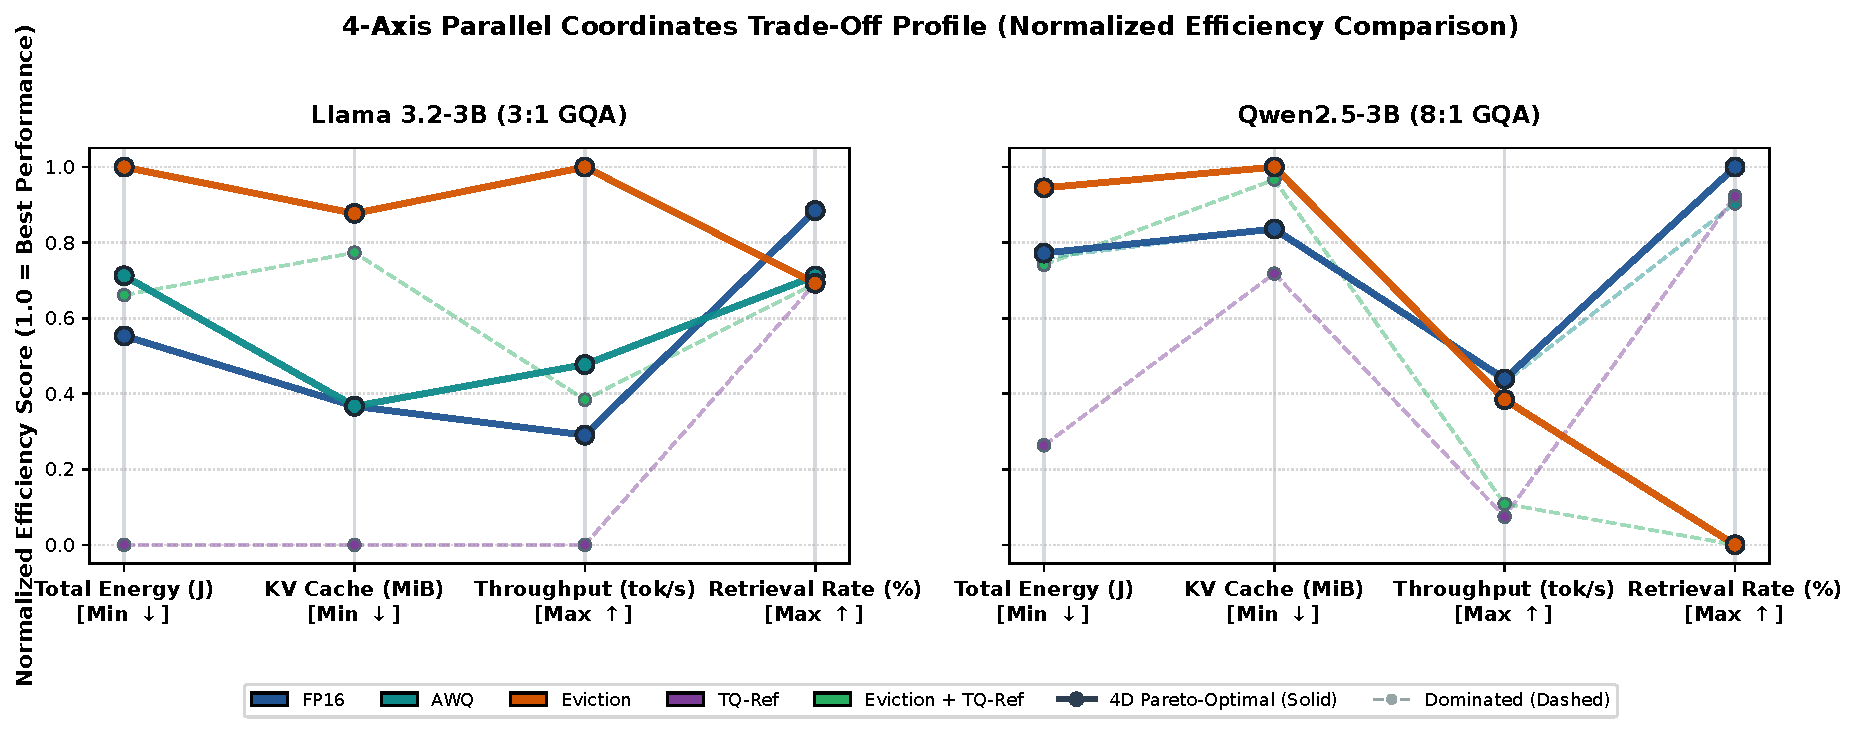
\includegraphics[width=\columnwidth]{figures/fig_pareto_4d_parallel_coords.pdf}
\caption{Four-axis parallel coordinates trade-off profile at 4096 tokens across total energy, KV cache footprint, decode throughput, and hard-retrieval accuracy for Llama~3.2-3B (left) and Qwen2.5-3B (right). Solid polylines indicate 4D Pareto-optimal configurations; dashed polylines denote dominated configurations.}
\label{fig:pareto4d}
\end{figure}

\begin{table}[t]
\caption{Four-Objective Pareto Frontier at 4096 Tokens (2000 Bootstrap Resamples)}
\label{tab:pareto4d}
\centering\footnotesize
\setlength{\tabcolsep}{1.25pt}
\renewcommand{\arraystretch}{0.80}
\begin{tabular*}{\columnwidth}{@{\extracolsep{\fill}}lrrr@{\hspace{0.85em}}cl@{}}
\toprule
\multicolumn{6}{c}{\textbf{Llama 3.2-3B (3:1 GQA)}} \\
\midrule
\textbf{Config} & \textbf{$E$ (J) $\downarrow$} & \textbf{KV $\downarrow$} & \textbf{tok/s $\uparrow$} & \textbf{Hits $\uparrow$} & \textbf{Status} \\
\midrule
FP16 (C0)      & $701.08 \pm 8.12$  & 455.0 & $11.34 \pm 0.06$ & 47/60 & \textbf{PF} 100.0\% \\
AWQ (C1-W)     & $639.86 \pm 5.48$  & 455.0 & $13.71 \pm 0.24$ & 38/60 & \textbf{PF} 65.5\% \\
Evict (C2)     & $529.30 \pm 20.02$ & 119.0 & $20.34 \pm 1.62$ & 37/60 & \textbf{PF} 100.0\% \\
TQ-Ref (C3)    & $913.48 \pm 2.11$  & 696.5 &  $7.66 \pm 0.02$ & 37/60 & Dom. \\
Comp. (C4)     & $659.50 \pm 21.35$ & 187.2 & $12.53 \pm 0.96$ & 37/60 & Dom. \\
\midrule
\multicolumn{6}{c}{\textbf{Qwen2.5-3B (8:1 GQA)}} \\
\midrule
\textbf{Config} & \textbf{$E$ (J) $\downarrow$} & \textbf{KV $\downarrow$} & \textbf{tok/s $\uparrow$} & \textbf{Hits $\uparrow$} & \textbf{Status} \\
\midrule
FP16 (Q0)      & $616.78 \pm 6.79$  & 146.2 & $13.23 \pm 0.15$ & 53/60 & \textbf{PF} 98.0\% \\
AWQ (Q1-W)     & $621.75 \pm 25.14$ & 146.2 & $13.12 \pm 1.03$ & 48/60 & Dom. \\
Evict (Q2)     & $550.48 \pm 10.07$ &  38.2 & $12.53 \pm 1.46$ & 1/60  & Fail \\
TQ-Ref (Q3)    & $812.28 \pm 13.11$ & 223.9 &  $8.54 \pm 0.20$ & 49/60 & Dom. \\
Comp. (Q4)     & $628.69 \pm 9.77$  &  60.2 &  $9.04 \pm 0.60$ & 1/60  & Fail \\
\bottomrule
\end{tabular*}

\vspace{1pt}
\raggedright\footnotesize KV cache is in MiB. Energy and throughput are mean $\pm$ SD. PF denotes Pareto-frontier membership; percentages report unconstrained bootstrap selection frequency. Dom. denotes dominated, and Fail denotes retrieval below 50\%.\par
\end{table}

For Llama, single-stage eviction (C2) provides the most favorable balance across system metrics: minimal total energy ($529.30$~J), smallest cache footprint ($119.0$~MiB), and maximal throughput ($20.34$~tok/s), while staying within one test case of baseline retrieval (37/60 vs.\ 38/60) with 100.0\% bootstrap selection stability. Uncompressed FP16 (C0, 100.0\%) and wrapped AWQ (C1-W, 65.5\%) remain on the Pareto frontier due to higher retrieval accuracy (78.3\% and 63.3\%). TurboQuant reference variants C3-Ref (0.0\%) and C4-Ref (35.2\%) are dominated. Single-stage eviction (C2) strictly outperforms compound stacking (C4-Ref) across all operational metrics (19.7\% lower energy, 62.3\% higher throughput, 36.4\% smaller cache at identical 37/60 retrieval).

For Qwen, uncompressed FP16 (Q0) is Pareto-optimal ($616.78$~J, $13.23$~tok/s, 88.3\% retrieval, 98.0\% stability), dominating wrapped AWQ (Q1-W, $621.75$~J, 80.0\% retrieval). Token eviction (Q2) appears on the unconstrained frontier in 100.0\% of resamples, with energy of $550.48$~J, cache of $38.2$~MiB, and retrieval of 1/60 (1.7\%). Under a practical viability threshold ($Q \ge 50\%$), Q2 is excluded, leaving Q0 as the sole viable frontier configuration.

\paragraph{Power Trace Robustness}
Raw NVML power traces exhibited transient excursions above the nominal 70~W cap, peaking at 124.5~W on Llama and 116.1~W on Qwen. Reintegrating traces after clipping samples at 82~W or 70~W preserved the energy ranking and registered significance decisions within each model.

%% ════════════════════════════════════════════════════════════════
%%  5. DISCUSSION AND LIMITATIONS
%% ════════════════════════════════════════════════════════════════
\section{Discussion and Limitations}

\subsection{Eviction Divergence and Architecture Sensitivity}
The primary divergence in our data is the sharp difference in retrieval retention under token eviction. Three factors may contribute.
(1)~\textbf{GQA Head Sharing:} One KV entry serves eight query heads on Qwen and three on Llama (Fig.~\ref{fig:eviction_gqa}).
(2)~\textbf{Tokenization Density:} Vocabulary size (152k vs.\ 128k), tokenization, and chat formatting can change which tokens fall within an observation window.
(3)~\textbf{Heuristic Portability:} Layer count (36 vs.\ 28), configured context length (32K vs.\ 128K), and model-specific adapters also differ and can affect the comparison.

\begin{figure}[t]
\centering
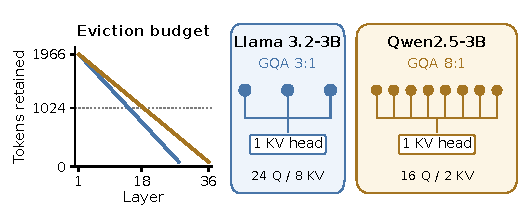
\includegraphics[width=\columnwidth]{figures/eviction_schedule_and_gqa.pdf}
\caption{PyramidKV-style budgets (mean 1024 tokens per layer) and query-to-KV head-sharing layouts for the two models. Each diagram shows one KV head and its associated query heads.}
\label{fig:eviction_gqa}
\end{figure}

The sensitivity sweep varies only the retained-token budget (Table~\ref{tab:qwen-sensitivity}). It establishes limited recovery over that range and leaves the contribution of GQA head sharing unresolved.

\subsection{Realization Gaps and Joint Rate-Distortion Optimization}
\label{sec:joint-opt}
We evaluated TurboQuant using its numerical reference implementation rather than a fused CUDA kernel. In reference form, retaining uncompressed tensors alongside discrete codebook indices added 31\% to 45\% energy overhead and increased memory footprint. Under our ideal packing assumptions, the non-evicted 4-bit decode cache would occupy 28.8\% of the corresponding FP16 cache. A production kernel that packs indices and fuses dequantization into attention would need separate hardware measurements.

These silicon measurements provide direct physical motivation for joint rate-distortion frameworks like RDKV~\cite{zhang_rdkv_2026} and ThinKV~\cite{ramachandran_thinkv_2026}. These frameworks motivate testing whether a joint policy can preserve retrieval while reducing the cost of sequential stages. In our runs, the compound stack consumed more energy than eviction alone. At the same time, the negative interaction ($I < 0$) shows that eviction reduced the incremental cost of TQ-Ref. The smaller retained cache is consistent with this result.

\subsection{Limitations and Threats to Validity}
\paragraph{Internal and Construct Validity} Measurements were gathered in continuous sessions on Google Colab with five independent blocks per condition ($n=5$). Llama systems contrasts use stock C1, with a separate wrapped control for the sensitivity check in Section~\ref{sec:interaction}. The Qwen AWQ comparisons use a common wrapper. All trace files were verified with SHA-256 checksums. Retrieval quality was evaluated via exact-match key-value extraction across three document depths; while this isolates cache retention, it does not assess multi-step dialogue. NVML power logging captures board-level GPU dissipation, excluding host CPU and system DRAM.
\paragraph{External and Statistical Validity} Experiments characterize two 3B models on a server-class NVIDIA T4. Edge accelerators differ in memory hierarchy, thermal envelope, and power management and require separate measurements. The cross-model comparison leaves GQA confounded with other architectural and implementation differences. Fixed 64-token decoding isolates compression mechanisms without modeling open-ended text generation. Family-wise error rates were controlled using Holm correction for energy contrasts and Bonferroni adjustments for McNemar tests.

%% ════════════════════════════════════════════════════════════════
%%  6. CONCLUSION AND REPRODUCIBILITY
%% ════════════════════════════════════════════════════════════════
\section{Conclusion and Reproducibility}

We evaluated multi-stage compression on two 3B models using 10~Hz T4 power traces and a calibrated 60-scenario retrieval benchmark. The measured trade-offs varied across models and context lengths. On Llama~3.2-3B, AWQ with PyramidKV-style eviction reduced energy by 16.15\%, increased throughput by 47.7\%, and decreased active cache by 73.8\% relative to stock AWQ at 4096 tokens. Retrieval stayed within one case of wrapped AWQ (37/60 vs.\ 38/60). The same policy dropped Qwen2.5-3B accuracy to 1/60 (from 48/60). The negative energy interactions indicate that eviction reduced the incremental cost of the TurboQuant reference path, which retained FP16 cache tensors. Future work should benchmark the pipeline on an edge accelerator, vary GQA head sharing in a controlled comparison, and measure a packed, fused KV quantization kernel.

Checkpoints, traces, scenarios, scripts, and notebooks will be released upon publication. Experiments used an NVIDIA Tesla T4 (40 SMs, 16~GB, 70~W), Linux x86\_64 kernel 6.6.122+, and an Intel Xeon CPU at 2.00~GHz. The stack comprised PyTorch 2.11.0+cu128, Transformers 5.12.1, CUDA 12.8, \texttt{gptqmodel==7.1.0}, \texttt{turboquant==0.2.0}, and \texttt{pynvml}.

%% ════════════════════════════════════════════════════════════════
%%  ACKNOWLEDGMENTS
%% ════════════════════════════════════════════════════════════════
\section*{Acknowledgment}
Generative AI assisted only with LaTeX formatting and document structure, not study design, data generation, analysis, or interpretation. The authors take full responsibility for the work.

%% ════════════════════════════════════════════════════════════════
%%  REFERENCES
%% ════════════════════════════════════════════════════════════════
\bibliographystyle{IEEEtran}
\IEEEtriggeratref{10}
\begingroup
\emergencystretch=1em
\bibliography{references}
\endgroup

\end{document}
